\documentclass[a4paper, 10pt]{report}
\usepackage[italian]{babel}
\usepackage[T1]{fontenc}
\usepackage[utf8]{inputenc}
\usepackage{charter}
\usepackage{amsmath}
\usepackage{amsthm}
\usepackage{amsfonts}
\usepackage{graphicx}
\usepackage{wrapfig}
\usepackage{tcolorbox}
\usepackage{fancyhdr}
\usepackage{listings}
\usepackage{longtable}

\usepackage{geometry}
\geometry{a4paper, left=2cm,right=2cm,top=2cm,bottom=2cm}

\pagestyle{fancy}
\lhead{}
\chead{}
\rhead{\bfseries 07 - 14 novembre 2019 }
\lhead{\bfseries Segnali e immagini}

\begin{document}
\subsection*{Trasformata di Fourier a tempo discreto}

\paragraph*{Campionamento} Sia $f(t)$ un segnale reale continuo, anche non periodico, con:
\begin{align*}
f: ]-\infty, +\infty[ \in R \rightarrow R
\end{align*}

\noindent e sia $s_{\Delta T}(t)$ un trano di impulsi (non espresso con serie di Fourier) di periodo $\Delta T$ (frequenza di campionamento $\mu_s = 1 / \Delta T$). Il \textbf{campionamento} di $f(t)$ sarà:
\begin{align*}
\tilde{f}(t) = f(t) \cdot s_{\Delta T}(t)
\end{align*}

\noindent ovvero consiste nella moltiplicazione del segnale per il treno di impulsi (in modo da discretizzarlo).

\paragraph*{Trasformata a tempo discreto} Data la trasformata di Fourier $F(\mu)$ di un segnale reale, la sua trasformata a tempo dscreto sarà:
\begin{align*}
\tilde{F}(\mu) = F(\mu) * S_{\Delta t}(\mu) &= \int^{+\infty}_{-\infty}F(\tau) S_{\Delta t}(\mu - \tau) \, dt \\
&= ...\\
&= \frac{1}{\Delta T} \sum^{+\infty}_{n = -\infty} F \left(\mu - \frac{n}{\Delta T}\right)
\end{align*}

\noindent\fbox{%
    \parbox{\textwidth}{%
        \begin{center}
        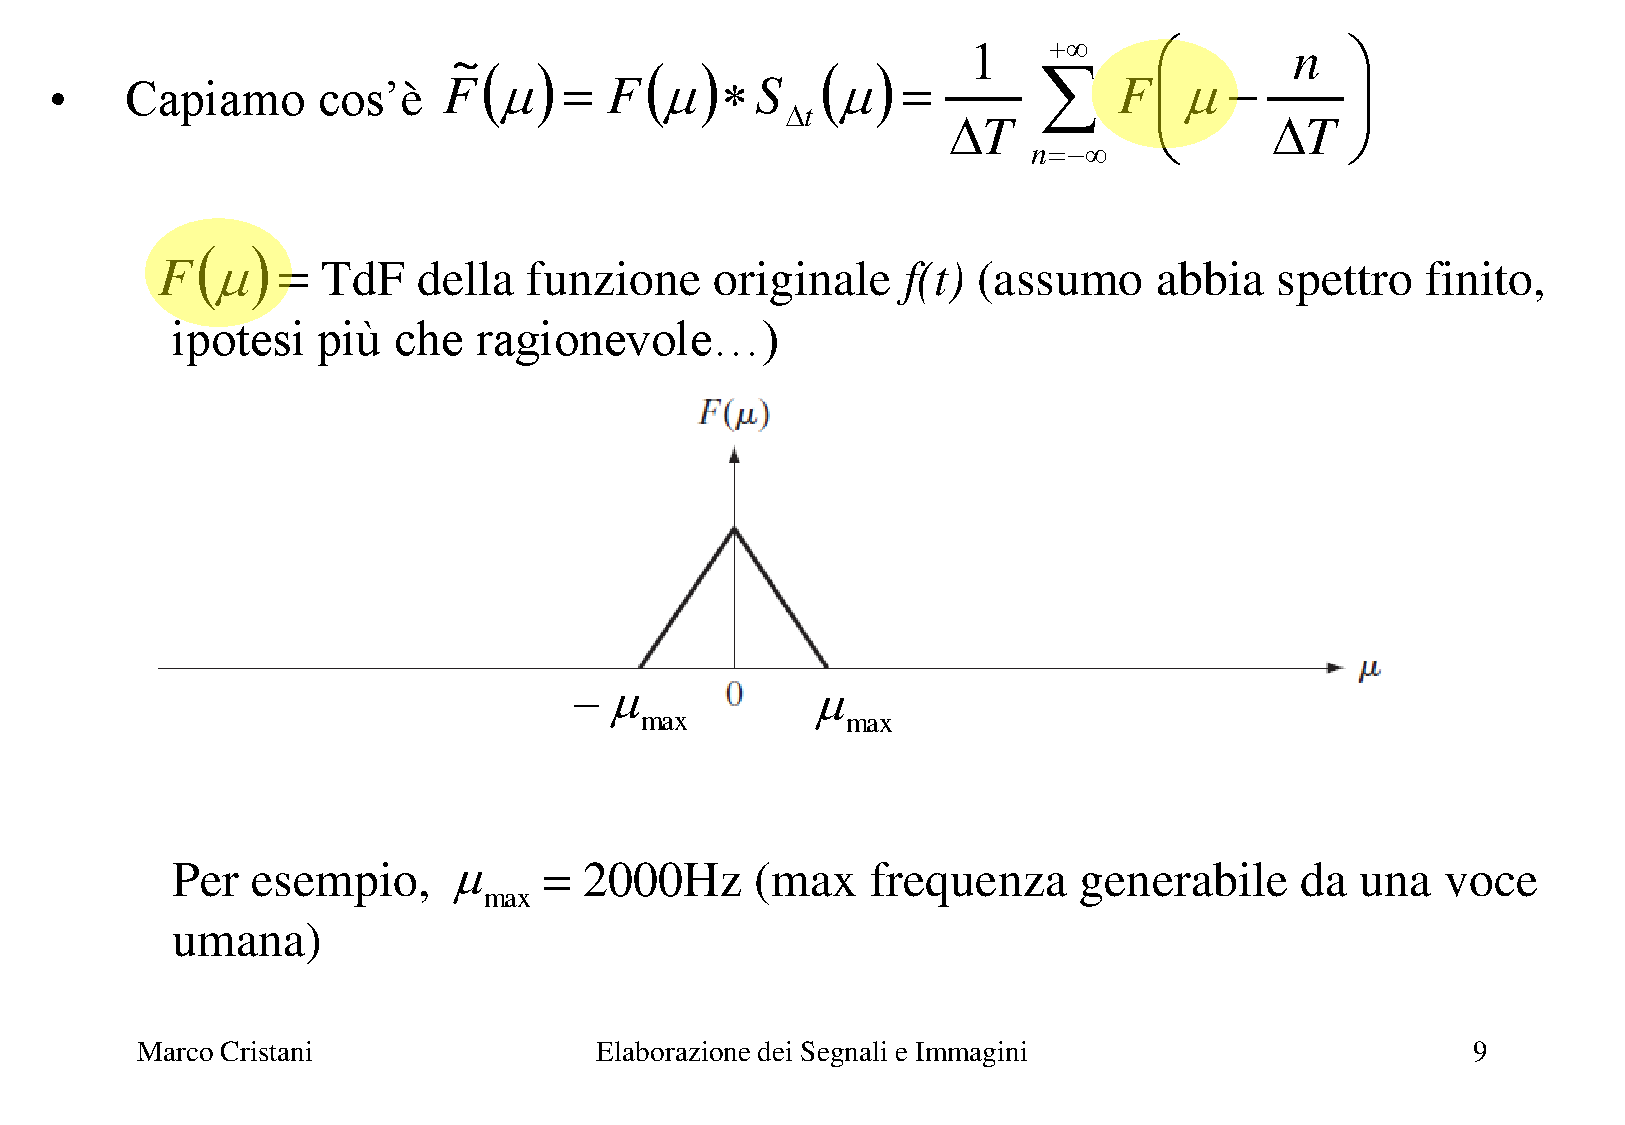
\includegraphics[scale=0.4]{1.pdf}
        \end{center}
    }%
}

\noindent\fbox{%
    \parbox{\textwidth}{%
        \begin{center}
        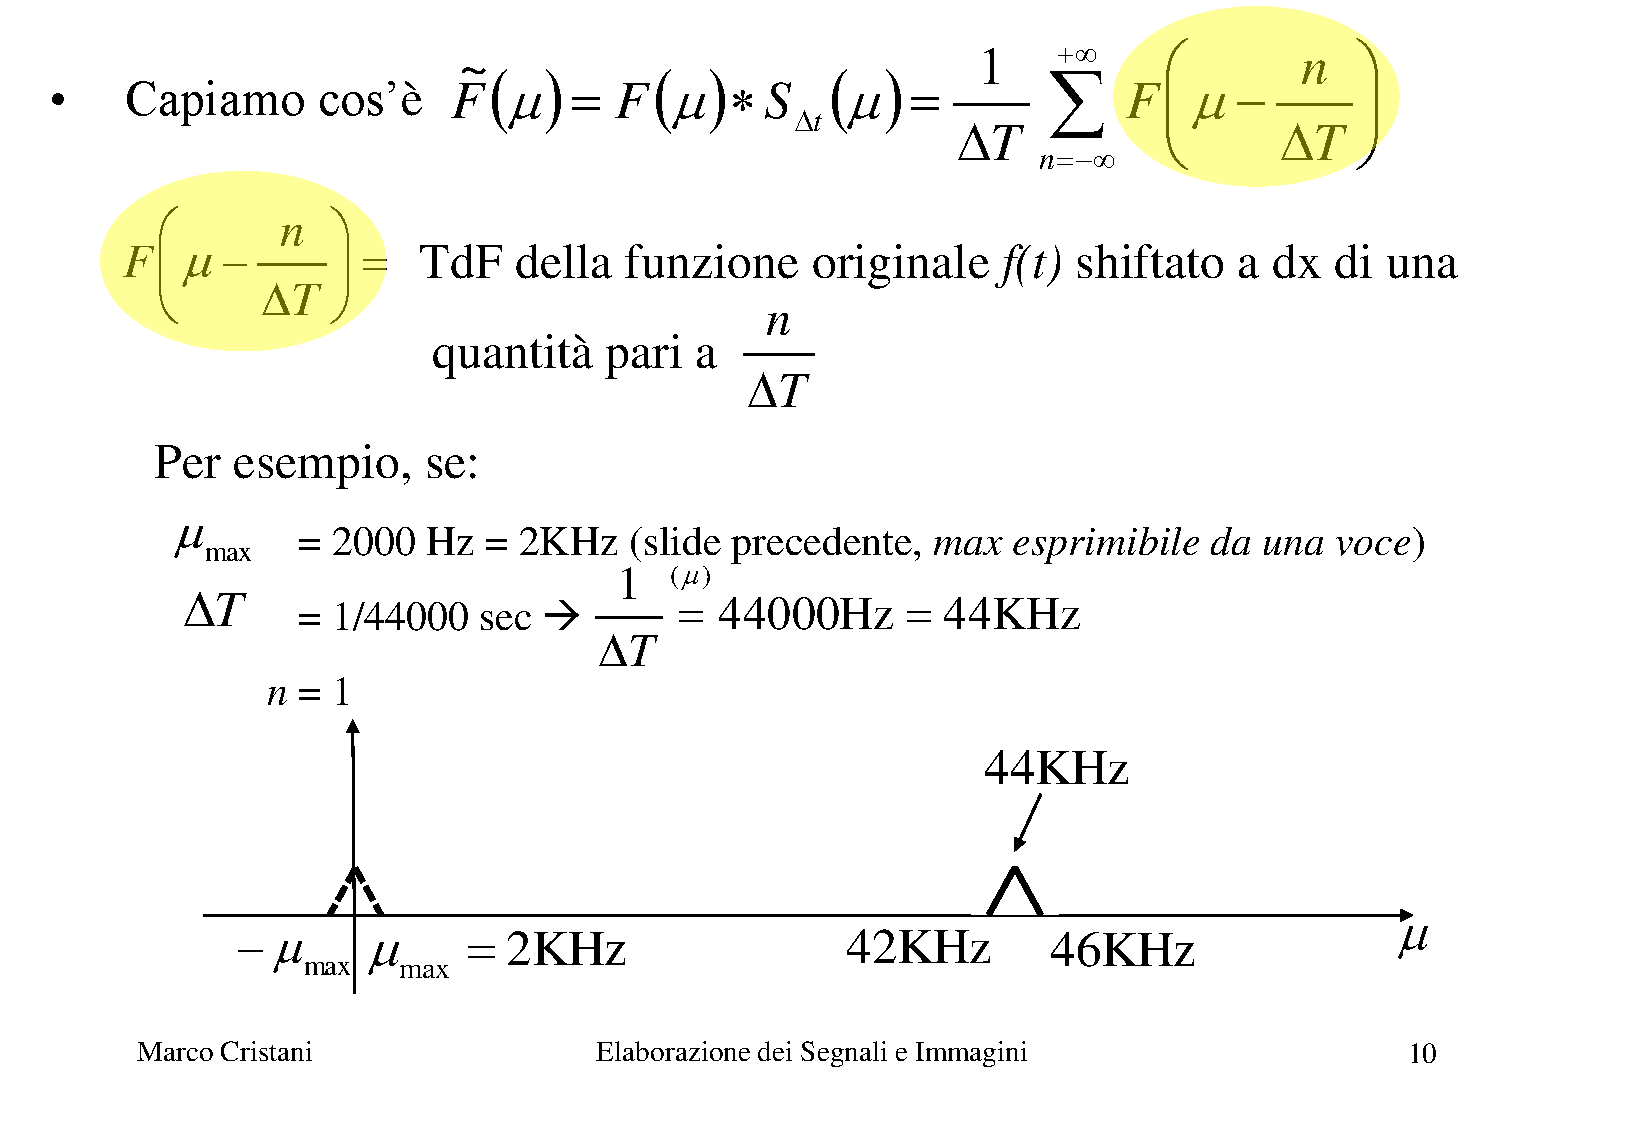
\includegraphics[scale=0.4]{2.pdf}
        \end{center}
    }%
}

\noindent\fbox{%
    \parbox{\textwidth}{%
        \begin{center}
        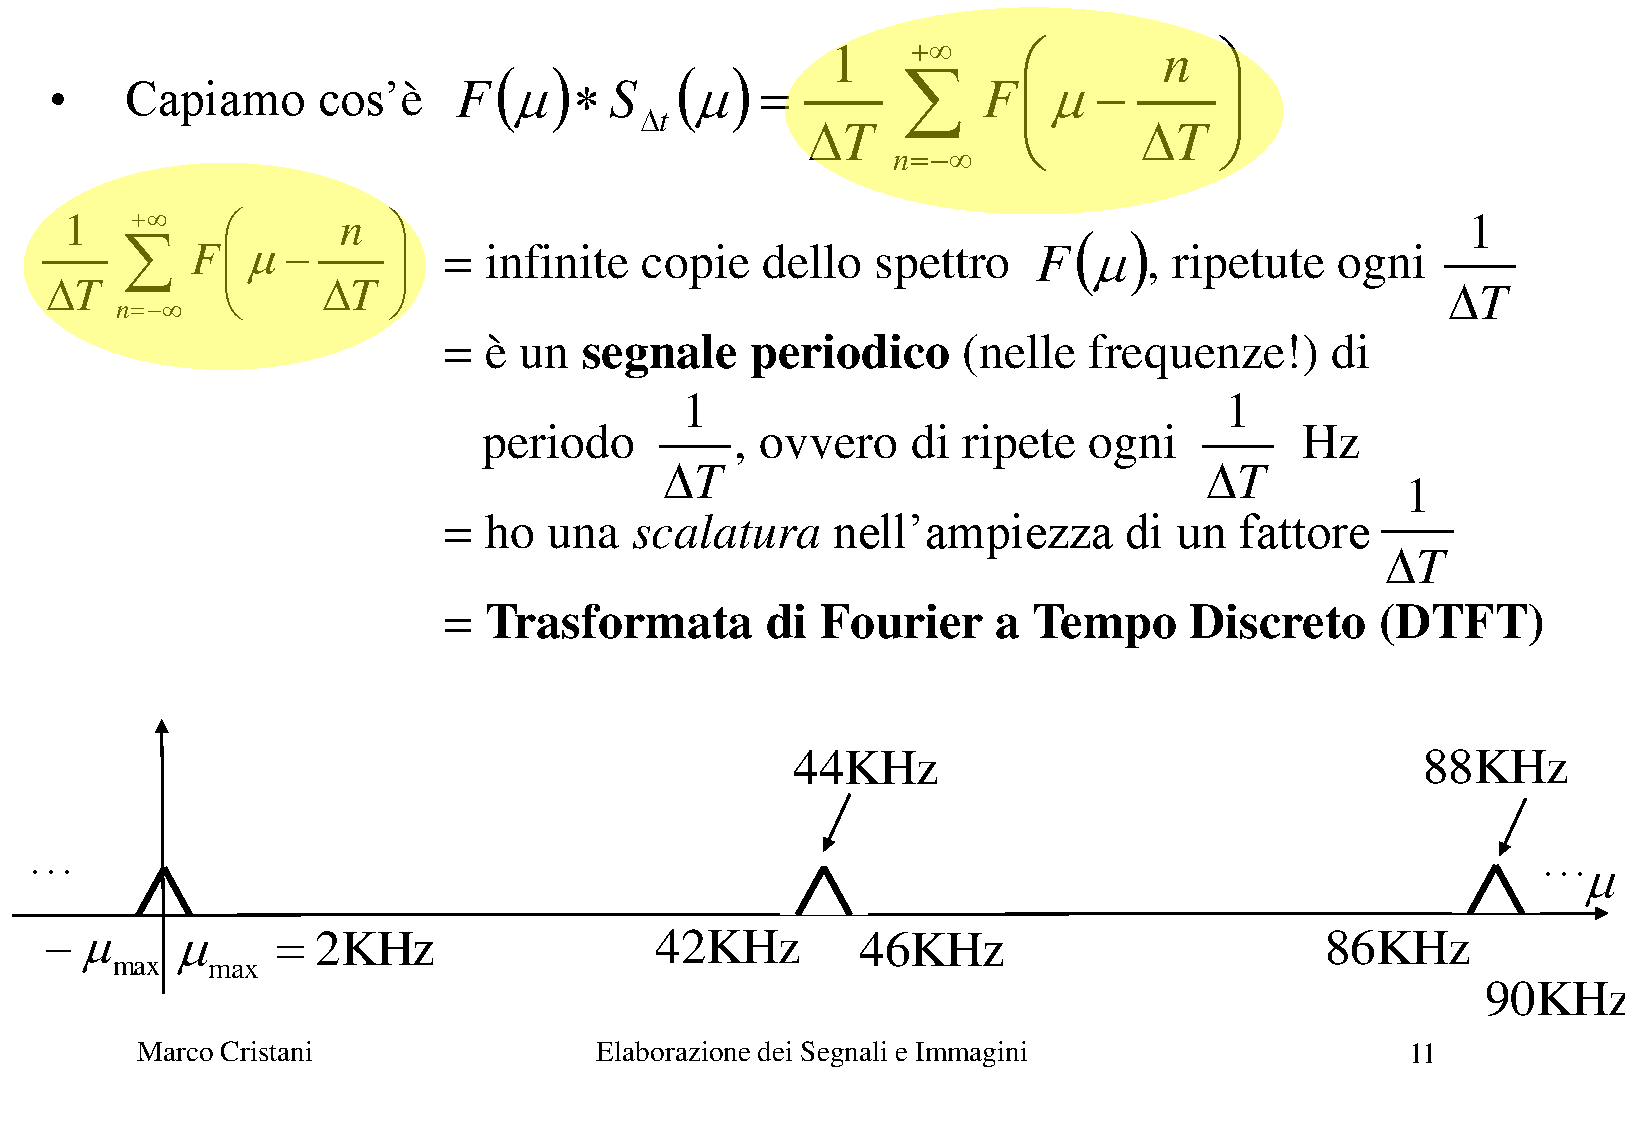
\includegraphics[scale=0.4]{3.pdf}
        \end{center}
    }%
}

\paragraph*{Teorema del campionamento} Un segnale reale continuo $f(t)$, limitato in banda, può essere riscotruito, completamente e senza errori, a partire da un insieme di suoi campioni selo se questi sono stati acquisiti con un tempo di campionamento $\Delta T$ tale per cui:
\begin{align*}
\mu_s > 2\mu_{MAX} \hspace{1cm}\text{con}\hspace{1cm} \mu_s = \frac{1}{\Delta T}
\end{align*}

\noindent Praticamente, per evitare l'aliasing (e quindi avere campioni corretti), devo ripetere il segnale con una frequenza maggiore a $2\mu_{MAX}$ (la "dimensione" del segnale è $\mu_{MAX}$ sinistro $+ \mu_{MAX}$ destro).\\

\noindent Il teorema del campionamento, in parole semplici, dice che tutte le proprietà di un segnale possono essere espresse dai suoi campioni.

\paragraph*{Ricostruzione del segnale} Dato un segnale campionato, la sua ricostruzione prevede 3 fasi:
\begin{enumerate}
\item Calcolo la trasformata di Fourier del segnale, da cui ottengo una funzione periodica (ogni periodo riporta una copia dello spettro della funzione continua);
\item Isolo un periodo della funzione;
\item Antitrasformo la sezione isolata.
\end{enumerate}



\noindent\fbox{%
    \parbox{\textwidth}{%
        \begin{center}
        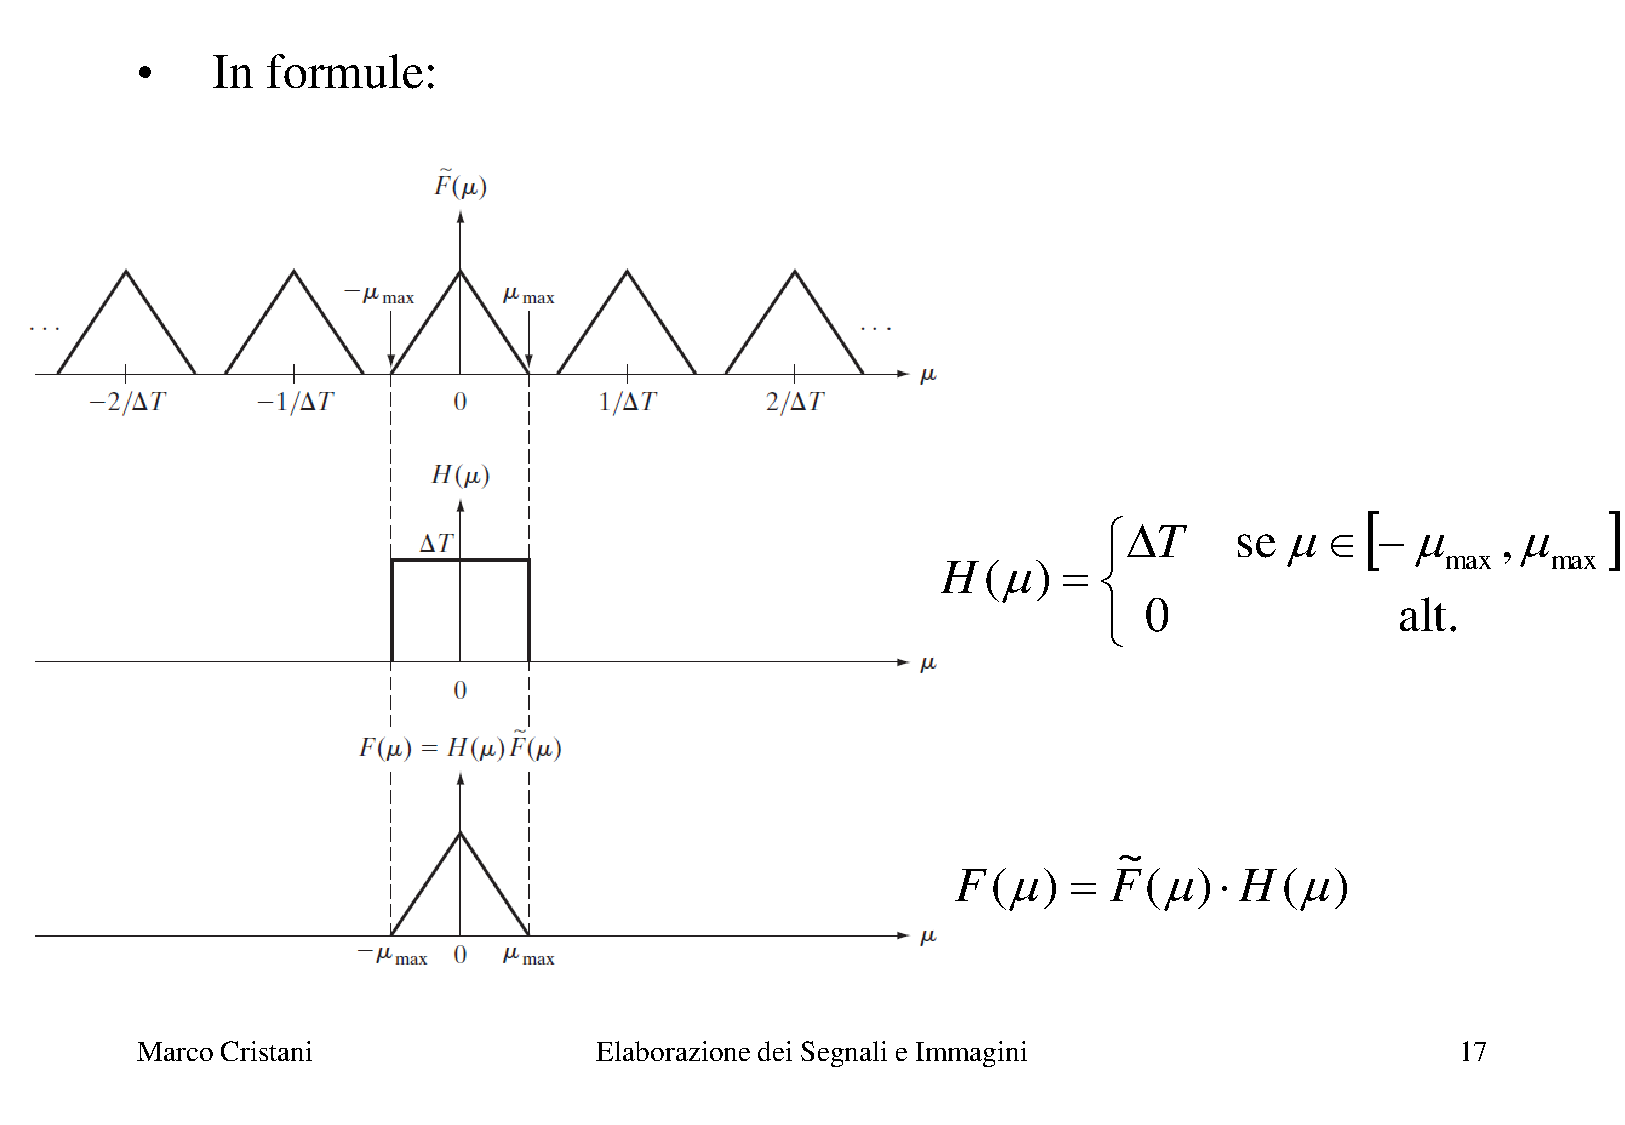
\includegraphics[scale=0.4]{5.pdf}
        \end{center}
    }%
}

\noindent Il calcolo per ricostruire il segnale è il seguente:
\begin{align*}
f(t) &= \mathfrak{F}^{-1}[F(\mu)]\\
&= \mathfrak{F}^{-1}[H(\mu)\tilde{F}(\mu)]\\
&= h(t) * \tilde{f}(t)
\end{align*}

\end{document}